\chapter{Time-resolved photoluminiscence of In$_{1-x}$Ga$_{x}$As$_y$Sb$_{1-y}$/GaAs/GaP QDs samples}

\section{Excitation density TRPL}
\label{chapter:appendix_TRPL_int}
\begin{figure}
	\centering
	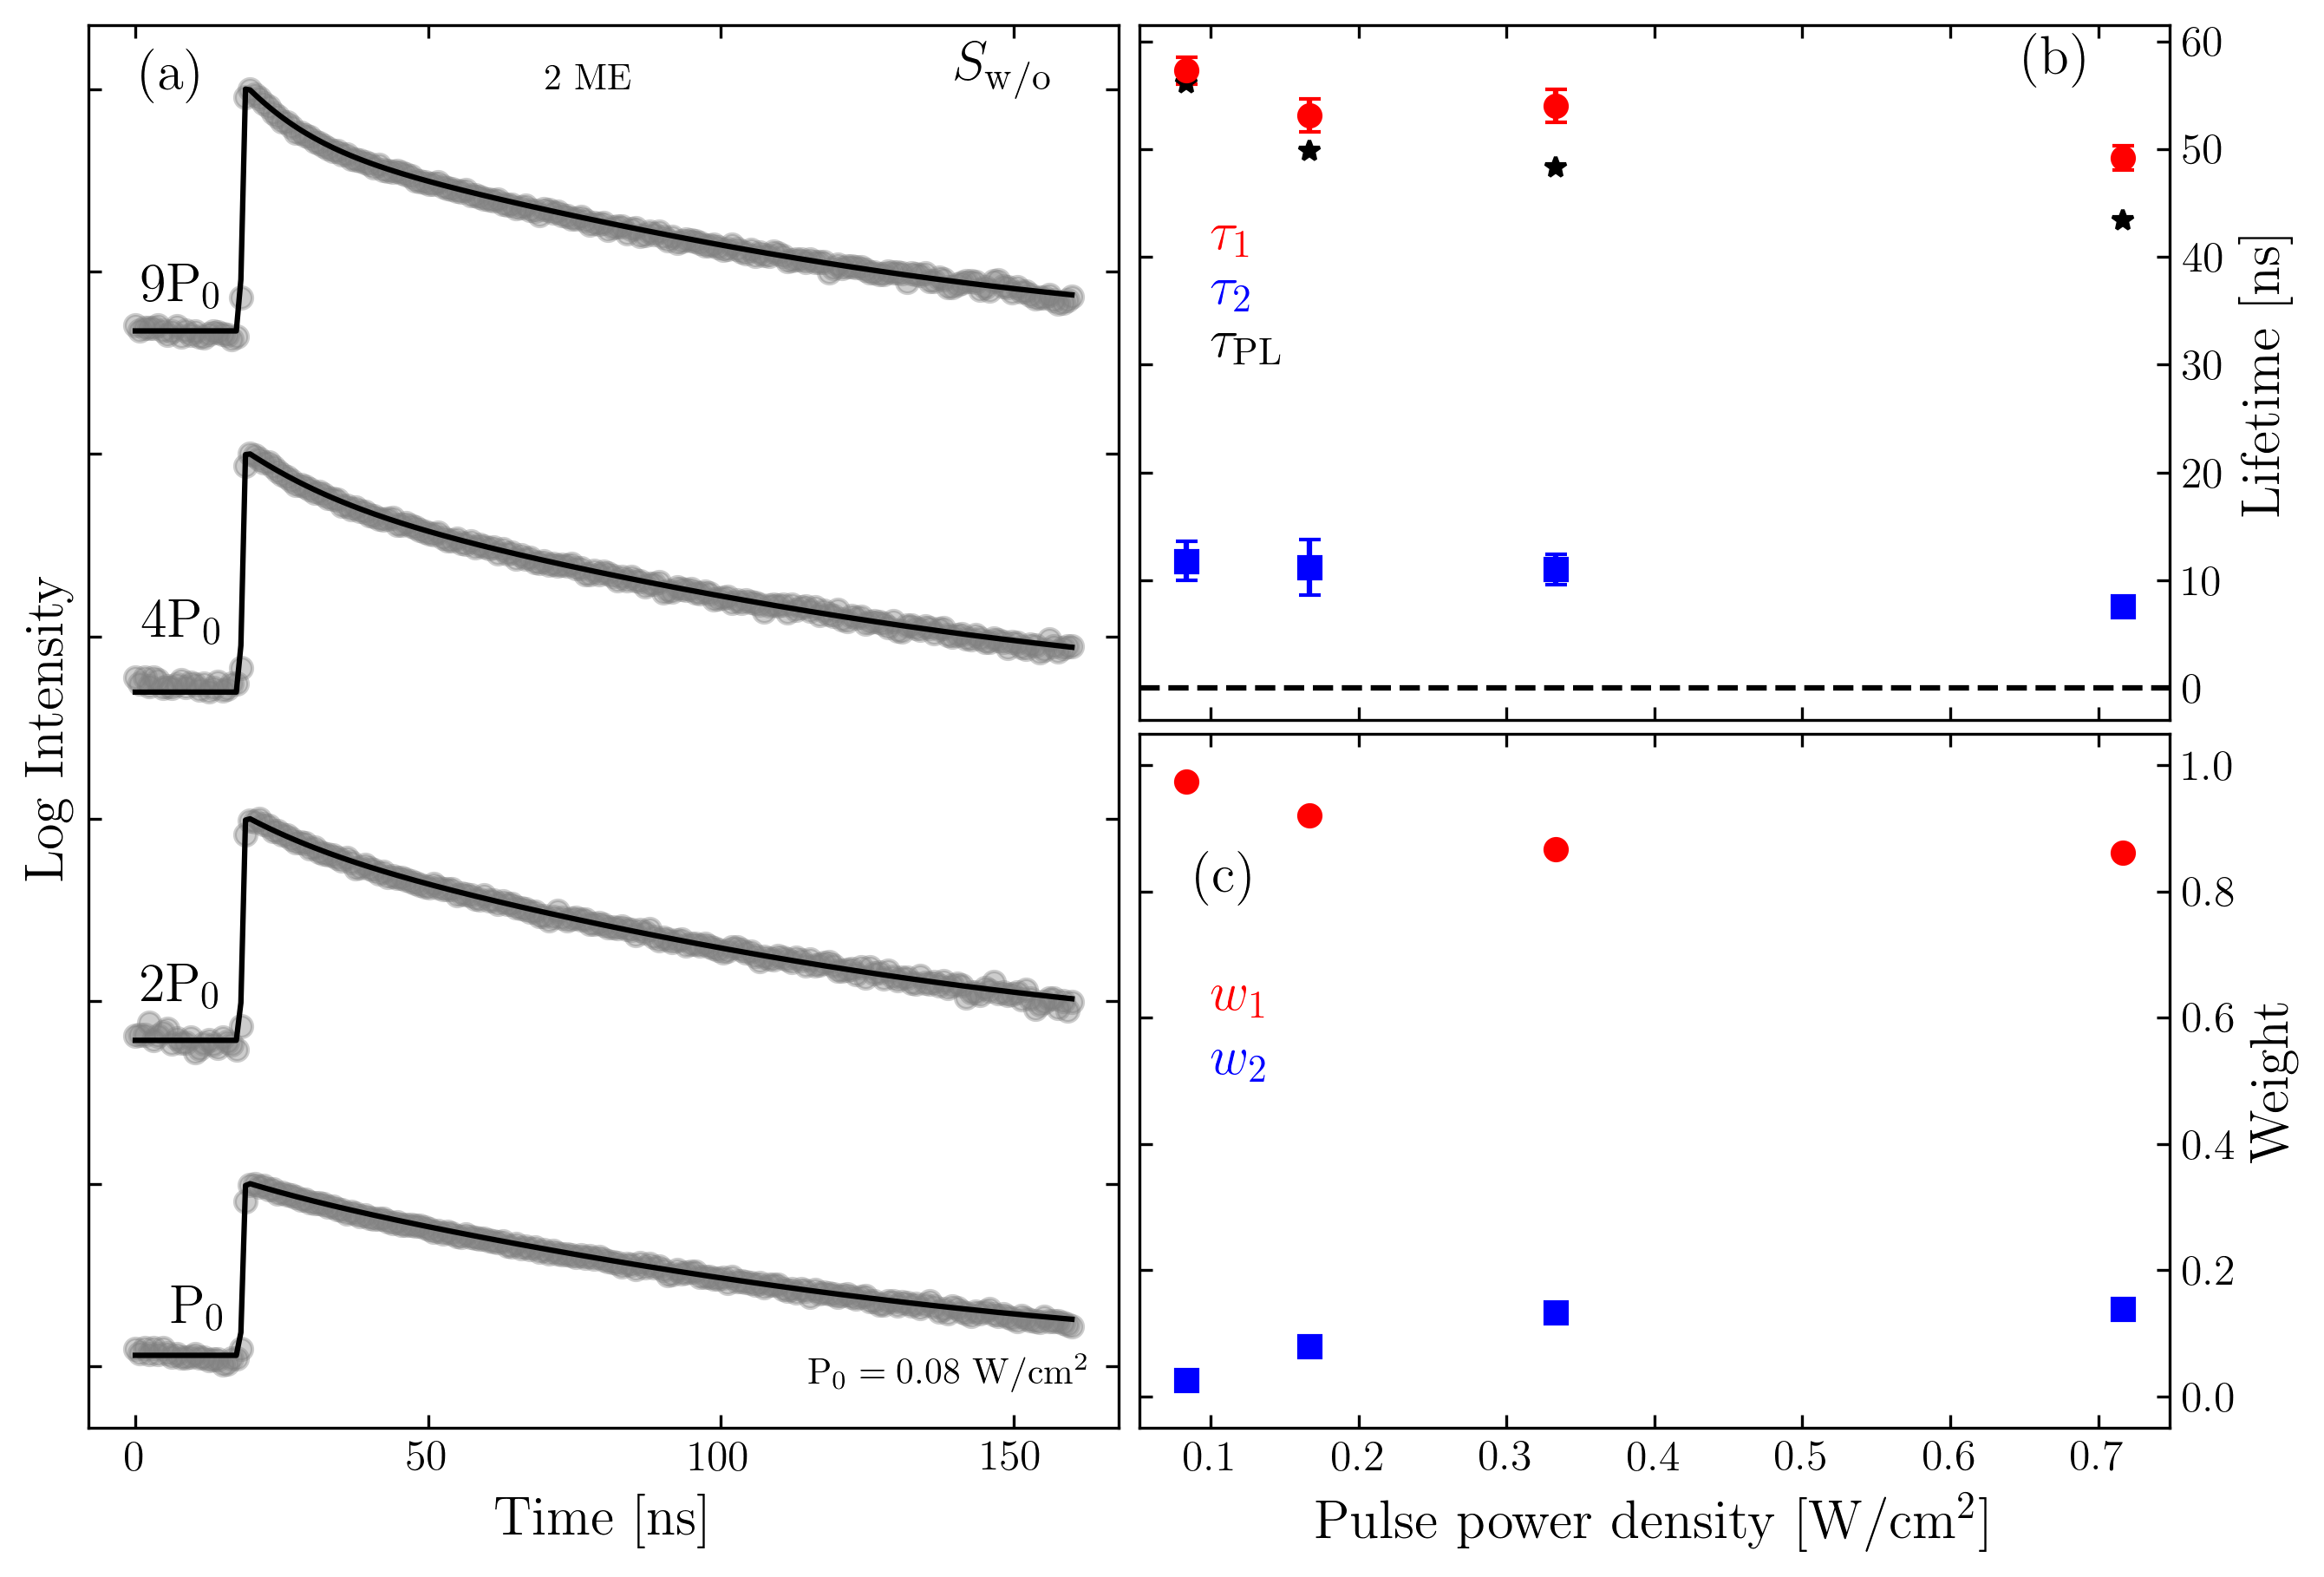
\includegraphics[width=0.9\linewidth]{/TRPL/intensity/12027_TRPL_max677_int}
	\caption{(a) TRPL measured at 15~K as a function of excitation density (grey circles) and its deconvolution by 2~ME model (solid lines) at the maximum of band $M_1^\mathrm{w/o}$ in the sample $S_\mathrm{w/o}$. (b) Fitted decay times $\tau_1$ (red circles), $\tau_2$ (blue squares) and characteristic time $\tau_\mathrm{PL}$ (black stars) as a function of excitation density. Appropriate weights are visualized in panel (c).}
	%\label{fig:TRPL_int_wo}
\end{figure}


\begin{figure}
	\centering
	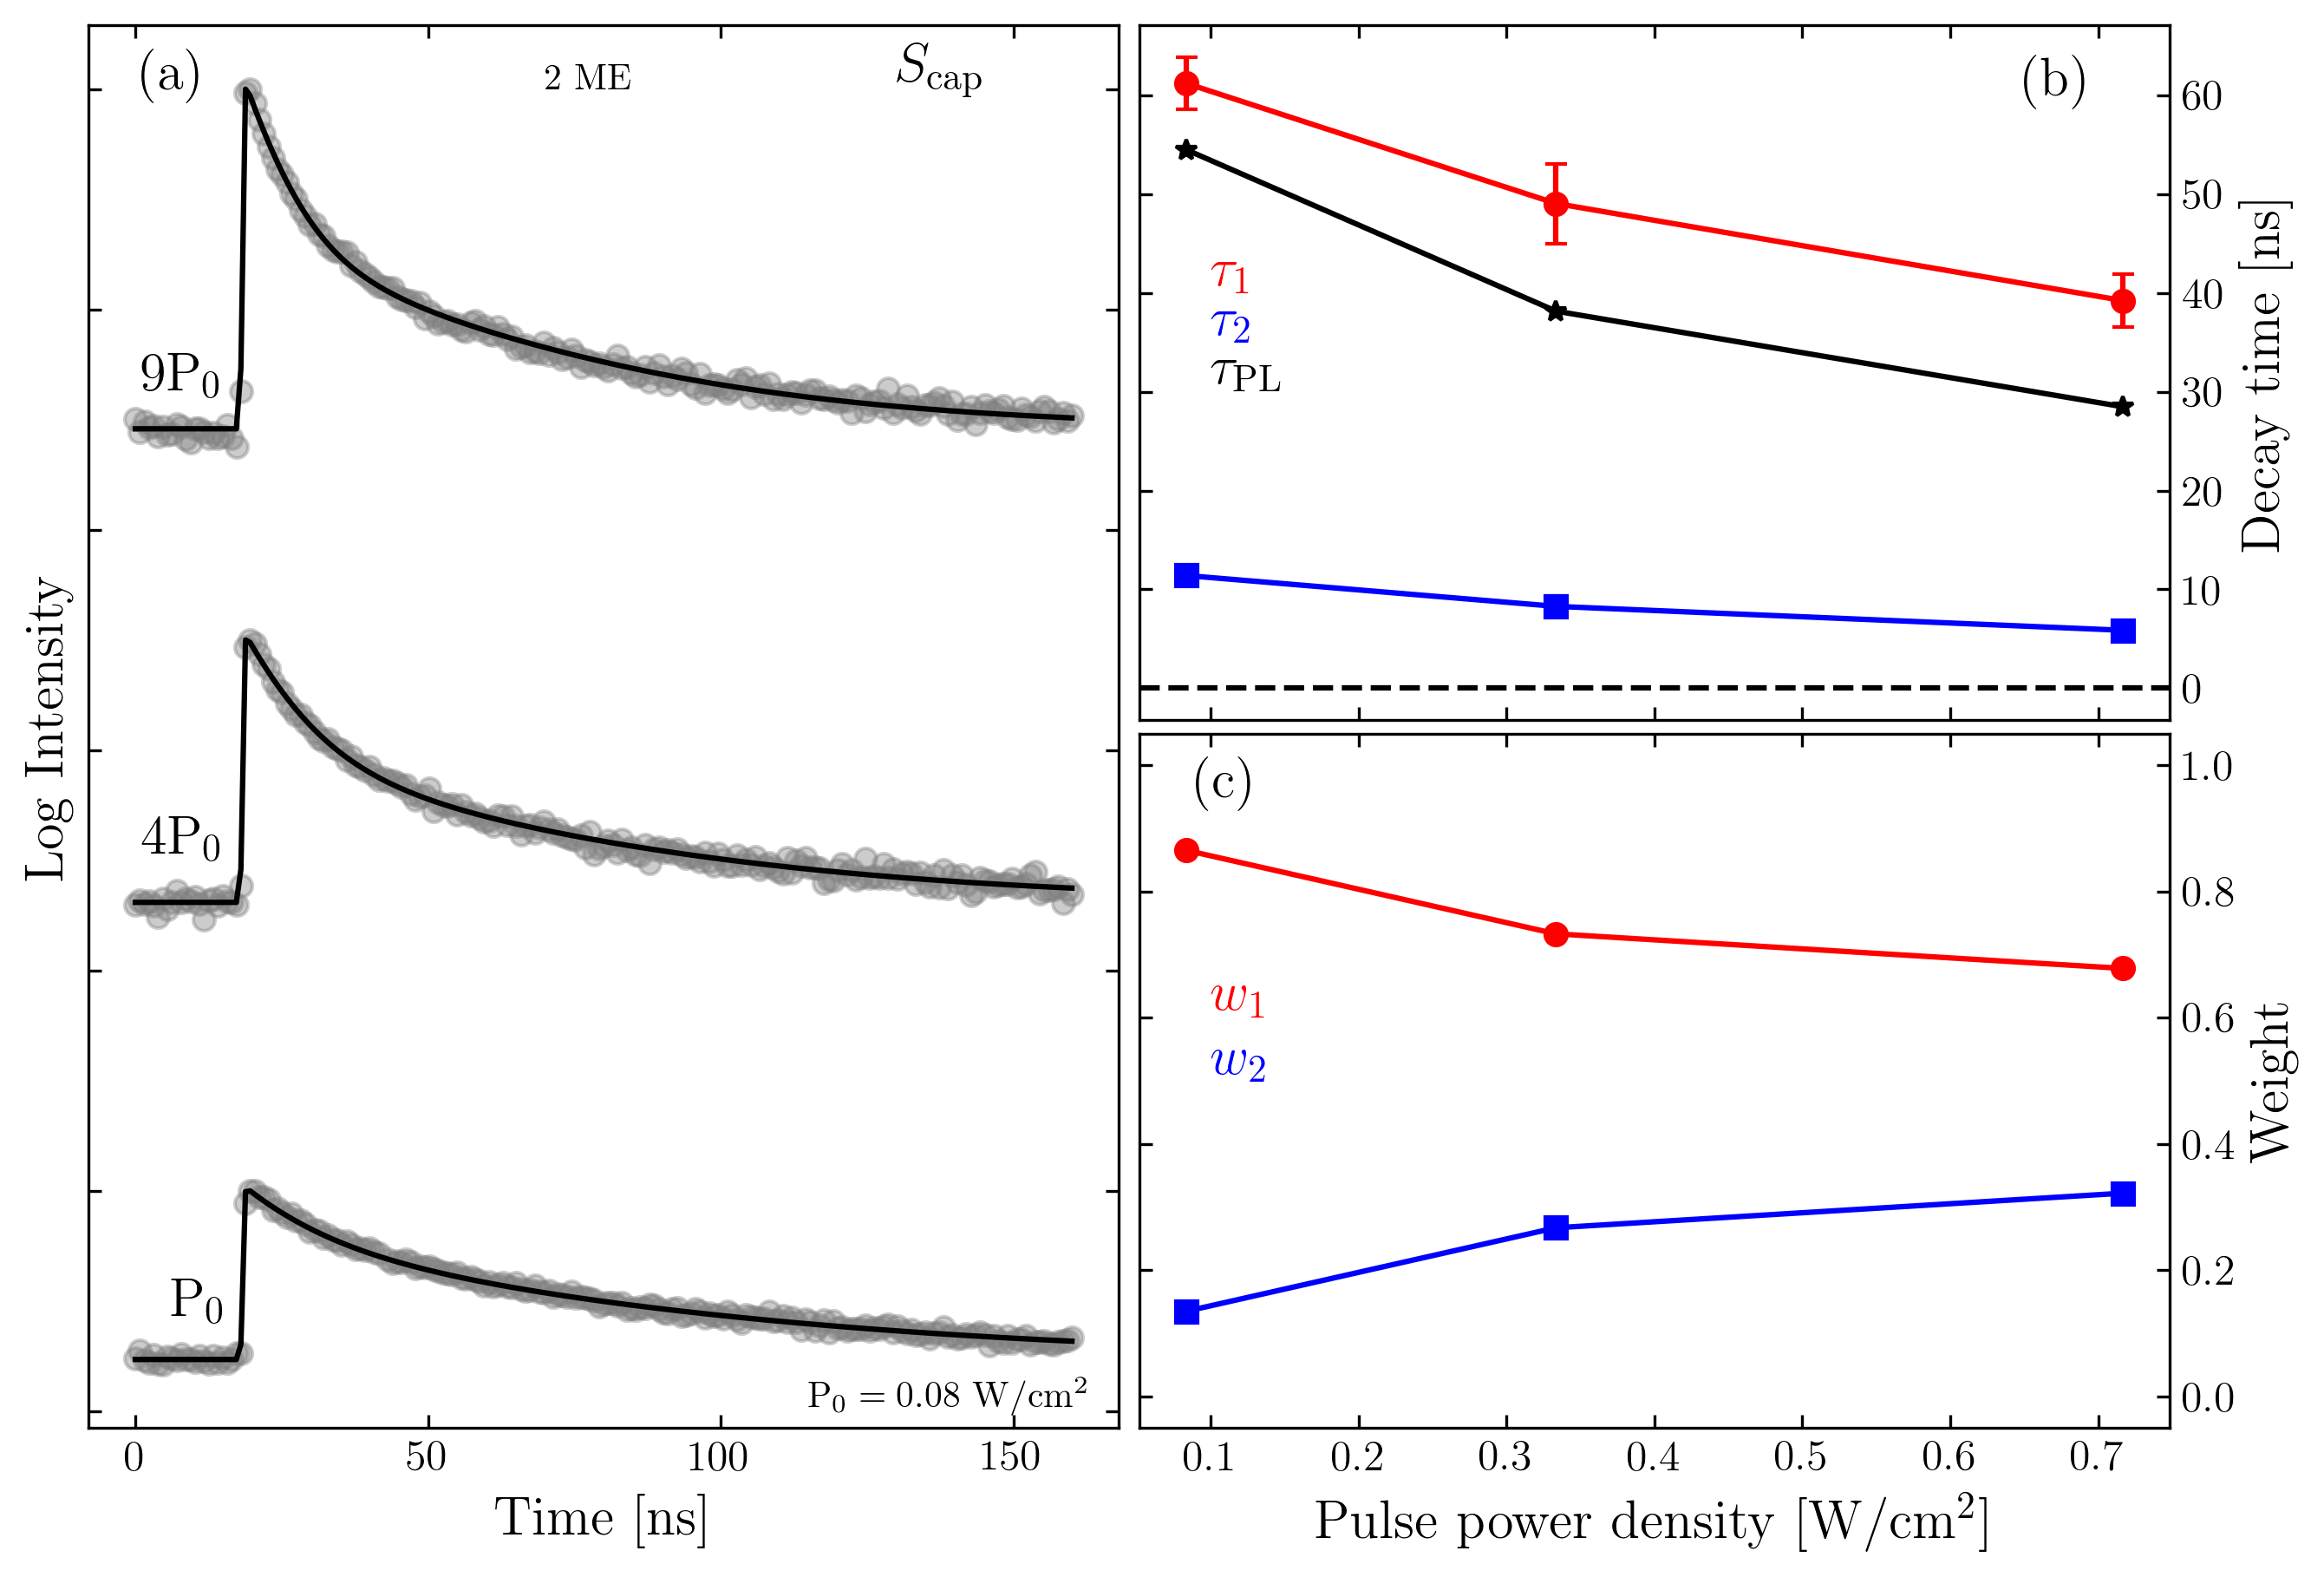
\includegraphics[width=0.9\linewidth]{/TRPL/intensity/12021_TRPL_max710_int}
	\caption{TRPL spectra of the maximum of band $M_1^\mathrm{c}$ in sample $S_\mathrm{cap}$. The results are given in the same nomenclature as in Fig.~\ref{fig:TRPL_temp_wo}.}
	%\label{fig:TRPL_int_c}
\end{figure}
\newpage 